% main.tex
\documentclass[12pt,a4paper]{report}

\usepackage{fontspec}
\defaultfontfeatures{Ligatures=TeX}
\setmainfont{Calibri}[
  Path=/Users/nchaikalis/Library/Fonts/,
  Extension=.ttf,
  UprightFont=Calibri,
  BoldFont=Calibrib,
  ItalicFont=Calibrii,
  BoldItalicFont=Calibriz
]
\setsansfont{Calibri}[
  Path=/Users/nchaikalis/Library/Fonts/,
  Extension=.ttf,
  UprightFont=Calibri,
  BoldFont=Calibrib,
  ItalicFont=Calibrii,
  BoldItalicFont=Calibriz
]
\setmonofont{Menlo}

\usepackage[a4paper,margin=2.5cm]{geometry}
\usepackage{setspace}
\usepackage{microtype}

\usepackage{graphicx}
\usepackage{booktabs}
\usepackage{longtable}
\usepackage{tabularx}
\usepackage{array}

\usepackage[hidelinks]{hyperref}

\setlength{\parskip}{0.6em}
\setlength{\parindent}{0pt}
\onehalfspacing

% Packages that must be in the preamble
% preamble.tex
\usepackage[acronym]{glossaries}
\usepackage{listings}
\lstset{
  basicstyle=\ttfamily\small,
  breaklines=true,
  frame=single,
  columns=fullflexible,
  keepspaces=true,
  showstringspaces=false
}
\makeglossaries


% Acronym definitions, still preamble safe
% glossaries.tex
% Acronym definitions for the thesis

\newacronym{rag}{RAG}{Retrieval Augmented Generation}
\newacronym{hyde}{HyDE}{Hypothetical Document Embeddings}
\newacronym{llm}{LLM}{Large Language Model}
\newacronym{nlp}{NLP}{Natural Language Processing}

\newacronym{api}{API}{Application Programming Interface}

\newacronym{doi}{DOI}{Digital Object Identifier}
\newacronym{pmid}{PMID}{PubMed Identifier}

\newacronym{vdb}{VDB}{Vector Database}

\newacronym{beir}{BEIR}{Benchmarking Information Retrieval}

\newacronym{ragas}{RAGAS}{Retrieval Augmented Generation Assessment}

\begin{document}

% Front matter
\pagenumbering{roman}
% frontmatter.tex
\begin{titlepage}
\begin{center}

{\large School of Medicine, MSc Biomedical Informatics, 2024 to 2026\par}
\vspace{1.0cm}

{\large School of Medicine\par}
{\large MSc Biomedical Informatics\par}
\vspace{1.0cm}

{\large Author: Nikolaos Chaikalis\par}
{\large Supervisor: Professor Eleni Kaldoudi\par}
{\large Supervising PhD Candidate: Nikolaos Portoakalidis\par}

\vspace{1.8cm}

{\LARGE Diploma Thesis\par}
\vspace{1.2cm}

{\Large
Design and Evaluation of a Retrieval Augmented Biomedical Platform for Thrombosis Risk Factor Extraction: Continuous PubMed Scheduling and Human in the Loop
\par}

\vfill

{\large June 2026\par}

\end{center}
\end{titlepage}

\chapter*{Abstract}
\addcontentsline{toc}{chapter}{Abstract}

Thrombosis is a major contributor to cardiovascular morbidity and mortality worldwide. Biomedical knowledge related to thrombosis risk factors evolves continuously through new scientific publications, yet clinicians and researchers primarily rely on static literature reviews and keyword based search systems. These traditional approaches lack semantic understanding, structured retrieval, automated knowledge freshness monitoring, and integrated validation workflows.

This thesis presents the design, implementation, and evaluation of a domain adapted Retrieval Augmented Generation platform tailored for thrombosis risk factor extraction from PubMed literature. The proposed system integrates semantic embedding based retrieval, vector database storage, configurable large language model generation, and a continuous DOI level ingestion scheduler. A human in the loop curation workflow is incorporated through annotation tooling, enabling validation and iterative improvement of extracted knowledge.

The platform follows modular architectural principles emphasizing reproducibility, observability, and configuration driven experimentation. A multi phase evaluation framework assesses retrieval quality, answer grounding, extraction accuracy, and operational reproducibility using qrels based ranking metrics, RAGAS metrics, extraction metrics, and recorded run artifacts. The June 2026 generation benchmark evaluates 25 thrombosis oriented questions across LLM only, RAG without HyDE, and RAG with HyDE modes, with extraction metrics reported only for the 13 questions that have derived gold factors, while the finalized June 2026 retrieval benchmark reports qrels based ranking metrics from a separate 25-query independent retrieval phase.
% evidence: evaluation_metrics/runs/old/june-07-valid-full-run-25-queries/20260605_123942_nogit/paper_benchmark_summary.json

The thesis contributes a reproducible biomedical RAG architecture, an incremental PubMed scheduling mechanism, a human in the loop integration pipeline, and a structured evaluation methodology. The empirical findings are interpreted conservatively: the platform demonstrates auditable experimental architecture and reproducible benchmark artifacts, not clinical readiness.

\clearpage

\chapter*{Acknowledgements}
\addcontentsline{toc}{chapter}{Acknowledgements}

I would like to express my sincere gratitude to my supervisor, Professor Eleni Kaldoudi, for her guidance, academic insight, and continuous support throughout the development of this thesis.

I also thank the supervising PhD candidate, Nikolaos Portoakalidis, for his constructive feedback and technical discussions during the implementation and evaluation phases.

I am grateful to the faculty and colleagues of the MSc Biomedical Informatics program for fostering an interdisciplinary academic environment.

Finally, I would like to thank my family and close friends for their continuous support and encouragement. I would also like to thank my dog for patiently tolerating the postponed walks and for providing moments of balance and perspective throughout this journey.

\clearpage


\tableofcontents
\cleardoublepage
\addcontentsline{toc}{chapter}{List of Figures}
\listoffigures
\cleardoublepage
\addcontentsline{toc}{chapter}{List of Tables}
\listoftables
\cleardoublepage

% Print acronyms here in front matter
\printglossary[type=\acronymtype,title=Acronyms]
\clearpage

% Main matter
\pagenumbering{arabic}

% chapter-01.tex
\chapter{Introduction}

\section{Background and Motivation}

Biomedical knowledge production has reached a scale that challenges conventional approaches to evidence access and synthesis. Clinicians, biomedical researchers, and applied data scientists routinely work in domains where relevant findings are distributed across large and constantly expanding publication streams. Under these conditions, the practical bottleneck is no longer simple document availability. The dominant challenge is the ability to identify relevant evidence, map it to a specific question, and preserve traceability between retrieved sources and generated analytical conclusions.

Traditional keyword search systems remain valuable for broad exploration and bibliographic retrieval, but they tend to degrade when user intent is semantically rich, context dependent, or expressed in non-standard terminology. In biomedical settings, this limitation is amplified by terminological variation, evolving nomenclature, and heterogeneous reporting styles across journals and subdisciplines. A question phrased from a clinical perspective may require retrieval of evidence described with mechanistic terminology, and vice versa. As a result, lexical matching alone often produces either incomplete recall or noisy result sets that increase downstream interpretation cost.

At the same time, standalone generative methods have introduced a second class of limitations. A model can produce fluent and coherent responses while remaining insufficiently anchored to verifiable evidence. For general-purpose tasks this may be acceptable in exploratory settings; for biomedical decision support it is not. Biomedical workflows require justifiable outputs, explicit provenance, and reproducible behavior under controlled conditions. Consequently, retrieval quality and generation quality cannot be evaluated independently if the system is intended for evidence-grounded use.

Retrieval Augmented Generation (RAG) has emerged as a response to this gap by coupling retrieval and synthesis within a single inference pipeline. In this paradigm, the model response is conditioned on context retrieved at query time, rather than relying exclusively on parametric memory. This coupling creates a stronger basis for verifiability because candidate evidence can be inspected and linked to answer content. For biomedical informatics, this is a meaningful shift: it aligns computational response generation with core requirements of evidence-aware reasoning, source transparency, and update sensitivity.

The motivation of this thesis is therefore not limited to building another search interface or another generative application. The central motivation is to define and evaluate a system architecture that can sustain continuous biomedical ingestion, semantically robust retrieval, and explicit evaluation of retrieval-generation behavior under reproducible experimental conditions. This motivation places architecture, operations, and evaluation methodology on equal footing. In this view, model quality is necessary but insufficient without lifecycle control and traceable measurement.

\section{Problem Statement}

This thesis addresses the integrated problem of continuous knowledge acquisition, structured indexing, and reproducible evaluation for biomedical question answering supported by retrieval augmentation. The emphasis on integration is essential. Each stage can be implemented in isolation, yet isolated optimization frequently produces systems that are difficult to validate, hard to compare, and fragile under operational change.

The first dimension of the problem concerns knowledge freshness. Biomedical evidence changes continuously, and any static corpus progressively diverges from current literature. A platform that cannot update systematically will eventually produce answers based on stale context, even when retrieval and generation components are individually strong. Freshness, therefore, is not a convenience feature; it is a validity requirement.

The second dimension concerns representational suitability for retrieval. New documents must be transformed into indexable units that preserve enough semantic signal for meaningful nearest-neighbor retrieval while remaining computationally tractable. This requires decisions about document granularity, metadata retention, and update semantics. Inadequate representation introduces hidden bias into retrieval, which then propagates into synthesis quality.

The third dimension concerns empirical validity. A system that produces compelling demonstrations but lacks reproducible evaluation procedures cannot support rigorous comparative analysis. Retrieval and generation behavior must be measured through repeatable experimental stages with preserved intermediate artifacts, so that observed performance can be interpreted as a property of the system configuration rather than an artifact of uncontrolled execution.

Existing approaches commonly privilege one dimension at the expense of the others. Static retrieval systems tend to support stable indexing but offer limited mechanisms for continuous acquisition. Standalone generative systems can deliver fluent responses but weaken evidence accountability when retrieval grounding is absent or inconsistent. Ad hoc evaluation scripts may provide snapshots of performance but often fail to preserve sufficient process traceability for robust replication. The central research problem of this thesis is therefore architectural: how to design a biomedical platform that unifies continuous ingestion, retrieval-grounded synthesis, and reproducible evaluation without collapsing these requirements into disconnected tooling.

\section{Research Objectives}

The first objective is to design a modular biomedical RAG architecture that separates acquisition, retrieval, synthesis, and evaluation concerns while preserving explicit integration boundaries. Modularity is treated as a methodological objective rather than only a software engineering preference. It enables controlled replacement of components, supports clearer attribution of observed behavior, and reduces confounding effects during comparative experimentation.

The second objective is to enable automated literature ingestion from PubMed through scheduled execution. This objective includes systematic handling of document identity through Digital Object Identifier (DOI) and PubMed Identifier (PMID) workflows, because identifier consistency directly affects deduplication, update tracking, and downstream reproducibility. Automated ingestion is framed here as a mechanism for maintaining evidence continuity, not merely as a convenience for operational automation.

The third objective is to define a reproducible evaluation framework for both retrieval and generation behavior. This objective requires stage-level artifact production, explicit run organization, and metrics-oriented execution paths that allow reanalysis. The intent is to ensure that reported behavior can be interpreted through transparent process history rather than isolated endpoint measurements.

The fourth objective is to support evidence-grounded question answering with configurable retrieval strategies, including Hypothetical Document Embeddings (HyDE), while preserving observability of system behavior. This objective introduces a deliberate tradeoff: advanced retrieval augmentation can improve semantic recall in difficult queries, yet it may increase latency variance and dependence on additional generation steps. The thesis therefore treats configurability and measurement as inseparable.

Collectively, these objectives prioritize scientific validity, reproducibility, and architectural clarity over isolated model-centric optimization. The expected outcome is a thesis-level research artifact in which design decisions can be connected to measurable system behavior with defensible methodological grounding.

\section{Contributions of the Thesis}

This thesis makes four principal contributions within the scope defined above. First, it contributes a system architecture for biomedical RAG that treats ingestion, retrieval, synthesis, and evaluation as coordinated subsystems rather than disconnected modules. The contribution is architectural: it specifies how component boundaries and interaction contracts can support both operational execution and research-grade analysis.

Second, it contributes an automated scheduling approach for recurrent PubMed ingestion. This contribution operationalizes continuous acquisition and directly addresses corpus staleness as a structural risk in biomedical question answering. By integrating scheduling with downstream ingestion workflows, the thesis frames freshness management as an architectural responsibility.

Third, it contributes a reproducible evaluation framework that structures retrieval and generation analysis into staged experimental pipelines. This contribution is methodological: it enables performance interpretation through preserved intermediate outputs and repeatable execution logic, thereby strengthening the internal validity of empirical conclusions.

Fourth, it contributes an empirical analysis framework for evidence-grounded answer generation under realistic operational constraints. The contribution is not presented as a claim of universal superiority over alternative systems; rather, it provides a controlled basis for discussing how architectural choices influence retrieval behavior, synthesis quality, and reproducibility characteristics.

These contributions are deliberately framed with conservative scope. The thesis does not claim to eliminate all limitations of biomedical question answering, nor does it claim generalization beyond the evaluated setup. Its contribution is a rigorously structured foundation for subsequent extension, replication, and comparative study.

\section{Thesis Structure}

The remainder of the thesis is organized to move from conceptual grounding to architectural definition, then to implementation and empirical analysis. Chapter 2 reviews related literature and establishes the scientific context for retrieval-augmented biomedical question answering. It clarifies how existing retrieval and generation paradigms motivate the architectural direction adopted in this work.

Chapter 3 presents the system architecture, including subsystem responsibilities, workflow design, and operational constraints. It explains why the platform is structured as coordinated services and how architectural tradeoffs are handled with respect to reproducibility, observability, and evidence grounding.

Chapter 4 describes implementation-level realization of the architecture. This chapter maps conceptual components to concrete service behavior and runtime orchestration choices, with emphasis on how the implemented system preserves the design intentions introduced earlier.

Chapter 5 defines the experimental methodology. It specifies evaluation objectives, experimental stages, and measurement strategy, so that empirical claims in later chapters can be interpreted within a transparent protocol rather than as isolated outcomes.

Chapter 6 reports evaluation results and examines retrieval and generation behavior through the defined methodology. The chapter emphasizes interpretation of system behavior in relation to architectural and pipeline decisions.

Chapter 7 provides discussion, including implications for biomedical information access and system design. It connects empirical findings to broader methodological questions about evidence grounding, reproducibility, and operational tradeoffs.

Chapter 8 addresses limitations and future work. It distinguishes current system boundaries from prospective extensions and clarifies which constraints arise from architecture, external dependencies, or evaluation scope.

Chapter 9 concludes the thesis by summarizing the problem framing, contributions, and principal findings. It restates the significance of integrating continuous ingestion, retrieval-grounded synthesis, and reproducible evaluation in a single biomedical platform.

This chapter progression is designed to preserve argumentative continuity: each chapter establishes prerequisites for the next, ensuring that final conclusions are grounded in explicit architectural reasoning and empirically traceable methodology.

% chapter-02.tex
\chapter{Background and Related Work}

\section{Biomedical Information Retrieval}

\section{Retrieval Augmented Generation in Biomedical Contexts}

\section{Risk Factor Extraction Literature}

\section{Knowledge Freshness and Incremental Ingestion}

\section{Human in the Loop NLP Systems}

\section{Related Work Comparative Matrix}
% chapter-03.tex
\chapter{System Architecture}

\section{Context and Architectural Scope}

This chapter defines the architecture of a platform that must support both continuous biomedical evidence acquisition and grounded analytical responses for thrombosis-oriented information needs. The architectural problem is not only to retrieve relevant literature, but to couple retrieval quality with lifecycle control, operational transparency, and experiment reproducibility. For this reason, the system is scoped as an integrated architecture rather than a single question answering service.

The platform is organized as three cooperating subsystems: a Biomedical Retrieval Augmented Generation (RAG) service, a PubMed scheduler service, and an evaluation subsystem used to execute comparative experiments. This scope establishes a full path from literature acquisition, to indexing and retrieval, to measured experimental outputs.
% evidence: biomed_knowledge_platform/src/biomed_platform/api/app.py
% evidence: scheduler_pubmed/src/api/app.py
% evidence: evaluation_metrics/src/phases/phase1_pool.py
% evidence: evaluation_metrics/src/phases/phase3_generate.py

This scope also establishes a separation between online inference concerns and experimental concerns. The biomedical RAG service is optimized for serving bounded-latency retrieval and synthesis requests, whereas the evaluation subsystem is designed to run multi-stage analyses that may be computationally intensive and asynchronous. The scheduler service bridges these two temporal scales by injecting new evidence into the retrieval corpus without requiring direct synchronization with user query timing.
% evidence: biomed_knowledge_platform/src/biomed_platform/api/endpoints/retrieval.py
% evidence: biomed_knowledge_platform/src/biomed_platform/api/endpoints/ask.py
% evidence: scheduler_pubmed/src/core/services/scheduler_runtime.py
% evidence: evaluation_metrics/src/phases/phase4_ragas.py

At repository level, this architecture is reflected in a monorepo with explicit subsystem boundaries. The biomedical RAG service and scheduler service are implemented as independent API applications with their own application and persistence lifecycles, the evaluation subsystem is implemented as a phase-oriented command-line pipeline, and the LLM server stack is separated as deployment infrastructure for model hosting. This organization expresses a deliberate architectural approach in which serving, orchestration, evaluation, and model-hosting responsibilities remain distinct while interoperating through explicit API contracts.
% evidence: biomed_knowledge_platform/src/biomed_platform/api/app.py
% evidence: biomed_knowledge_platform/src/biomed_platform/core/use_cases/ingestion.py
% evidence: biomed_knowledge_platform/src/biomed_platform/adapters/qdrant/vector_index.py
% evidence: scheduler_pubmed/src/api/app.py
% evidence: scheduler_pubmed/src/core/use_cases/scheduler.py
% evidence: evaluation_metrics/src/eval_cli.py
% evidence: llm_server/docker-compose.yml

The architectural implication of this monorepo structure is controlled evolution. Subsystems can evolve at different rates without forcing tightly coupled release behavior, while shared evaluation contracts preserve comparability across runs. In practice, this supports maintainability by localizing change impact and supports reproducibility by preserving stable boundaries between acquisition, retrieval, and evaluation concerns.

\section{Architectural Drivers and Constraints}

The dominant architectural driver is reproducibility. System behavior must be inspectable through explicit job states, persistent run records, and staged evaluation artifacts so that observed performance can be interpreted as the result of identifiable processing decisions. This requirement motivates asynchronous job orchestration and explicit persistence of both operational and experimental outputs.
% evidence: biomed_knowledge_platform/src/biomed_platform/core/domains/ingestion.py
% evidence: biomed_knowledge_platform/src/biomed_platform/core/use_cases/ingestion.py
% evidence: scheduler_pubmed/src/core/domains/scheduler.py
% evidence: evaluation_metrics/src/phases/phase1_pool.py
% evidence: evaluation_metrics/src/phases/phase4_ragas.py

A second driver is traceability across subsystem boundaries. Scheduler decisions, ingestion outcomes, and retrieval outputs must remain linkable so that failure analysis and evaluation interpretation can be performed without implicit assumptions. The architecture therefore favors explicit state transitions and structured interfaces over opaque internal coupling.
% evidence: scheduler_pubmed/src/core/use_cases/scheduler.py
% evidence: biomed_knowledge_platform/src/biomed_platform/api/endpoints/ingestion.py
% evidence: biomed_knowledge_platform/src/biomed_platform/core/use_cases/search.py

External dependency constraints are also central. The platform depends on remote biomedical data services, vector infrastructure, and generation infrastructure; consequently, readiness semantics, timeout handling, and controlled retry behavior are architectural requirements rather than implementation details. The tradeoff is additional operational complexity in exchange for bounded failure behavior.
% evidence: biomed_knowledge_platform/src/biomed_platform/core/services/readiness.py
% evidence: biomed_knowledge_platform/src/biomed_platform/adapters/pubmed/pubmed_client.py
% evidence: biomed_knowledge_platform/src/biomed_platform/adapters/qdrant/vector_index.py
% evidence: biomed_knowledge_platform/src/biomed_platform/adapters/ollama/ollama_client.py

Queue capacity and worker parallelism are additional constraints that influence ingestion throughput and failure handling semantics. The architecture therefore includes explicit backpressure behavior and retry-after signaling assumptions, so that ingestion acceptance remains predictable under bursty workloads. This choice constrains unbounded resource growth and supports operational stability, while making ingestion completion latency variable under load.
% evidence: biomed_knowledge_platform/src/biomed_platform/core/services/ingestion/backpressure.py
% evidence: biomed_knowledge_platform/src/biomed_platform/core/services/ingestion/in_memory_queue.py
% evidence: biomed_knowledge_platform/src/biomed_platform/api/app.py

\section{High Level Architecture}

At the system level, the architecture separates acquisition, retrieval, and evaluation concerns into distinct services with explicit interfaces. The biomedical RAG service exposes ingestion, retrieval, synthesis, and document management capabilities through an Application Programming Interface (API). The scheduler service governs periodic and manual acquisition workflows. The evaluation subsystem executes phase-based pipelines that query the API and materialize experiment artifacts.
% evidence: biomed_knowledge_platform/src/biomed_platform/api/endpoints/ingestion.py
% evidence: biomed_knowledge_platform/src/biomed_platform/api/endpoints/retrieval.py
% evidence: biomed_knowledge_platform/src/biomed_platform/api/endpoints/ask.py
% evidence: biomed_knowledge_platform/src/biomed_platform/api/endpoints/documents.py
% evidence: scheduler_pubmed/src/api/endpoints/scheduler.py
% evidence: scheduler_pubmed/src/api/endpoints/runs.py
% evidence: evaluation_metrics/src/phases/phase1_pool.py
% evidence: evaluation_metrics/src/phases/phase2_beir.py
% evidence: evaluation_metrics/src/phases/phase3_generate.py

\begin{figure}[h]
\centering
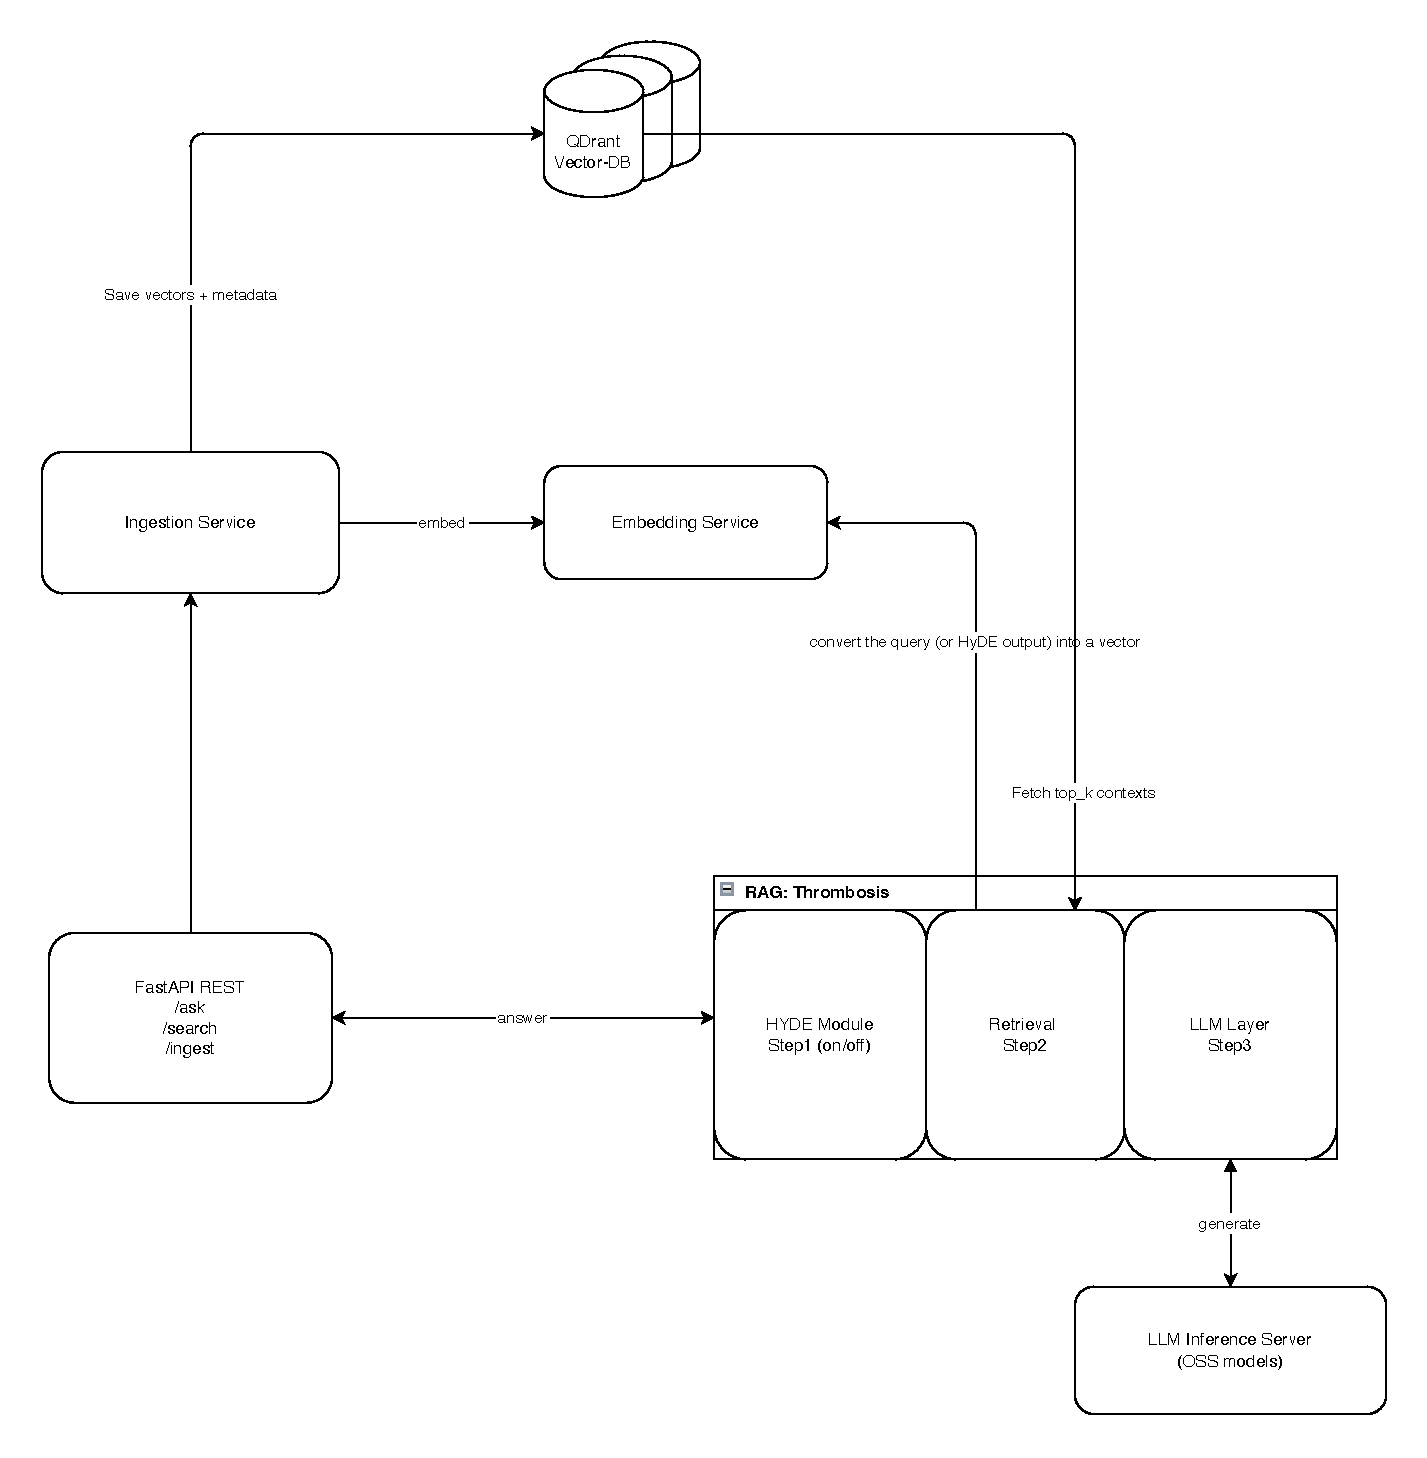
\includegraphics[width=0.9\linewidth]{resources/images/HLD.pdf}
\caption{High level architecture of the platform.}
\label{fig:architecture-high-level}
\end{figure}

Figure~\ref{fig:architecture-high-level} summarizes this decomposition and highlights a key design decision: scheduler execution and query-serving execution are operationally decoupled. This limits failure propagation across subsystems, but introduces eventual consistency between newly acquired literature and immediately retrievable indexed content.

\subsection{Subsystem Boundaries}

The high-level topology also reflects a contract-oriented integration strategy. The scheduler does not directly manipulate vector storage; instead, it communicates with the biomedical RAG service through documented endpoints for document existence checks, batch fetch, and ingest-job status tracking. This preserves ownership boundaries and reduces cross-service schema leakage, at the cost of additional network round-trips and stricter interface-version management.
% evidence: scheduler_pubmed/src/adapters/rag/documents_client.py
% evidence: scheduler_pubmed/src/core/ports/documents_client.py
% evidence: biomed_knowledge_platform/src/biomed_platform/api/endpoints/documents.py
% evidence: biomed_knowledge_platform/src/biomed_platform/api/endpoints/ingestion.py

\section{Human-in-the-Loop Curation Subsystem}

Label Studio is positioned in this architecture as a human-in-the-loop curation subsystem rather than as a core retrieval or answer-generation service. Its role is to host clinician-facing review tasks derived from candidate biomedical abstracts, while the surrounding \texttt{labelstudio-tools} package prepares tasks for upload, exports reviewed tasks, enriches them with bibliographic metadata, and hands curated records to the biomedical RAG ingestion API. This placement preserves a clean separation between evidence curation and online retrieval, while still allowing curated judgments to influence what enters the indexed corpus and what can later be used for evaluation-oriented analysis.
% evidence: labelstudio-tools/src/app/python/main.py
% evidence: labelstudio-tools/src/app/python/uploader.py
% evidence: labelstudio-tools/src/app/python/download_data/main.py
% evidence: labelstudio-tools/src/app/python/rag_importer/rag_integration.py

Architecturally, this subsystem sits between manual biomedical validation and downstream ingestion. Upstream, Excel-based abstract collections are loaded, optional exclusion filters are applied, and valid rows are transformed into Label Studio task payloads containing at minimum PMID, title, and abstract fields. Downstream, exported tasks are enriched with DOI and source metadata, partitioned into clean and rejected datasets according to ingestion requirements, and then transformed into batch ingestion requests for the biomedical RAG service. The resulting workflow constrains human review to a dedicated curation surface while keeping ingestion contracts explicit and machine-verifiable.
% evidence: labelstudio-tools/src/app/python/data_loader.py
% evidence: labelstudio-tools/src/app/python/filters.py
% evidence: labelstudio-tools/src/app/python/tasks.py
% evidence: labelstudio-tools/src/app/python/download_data/doi_enrich_any.py
% evidence: labelstudio-tools/src/app/python/download_data/main.py
% evidence: labelstudio-tools/src/app/python/rag_importer/rag_integration.py

This curation layer also has methodological significance for later evaluation chapters. The exported task structure retains manual annotation content alongside bibliographic identifiers and enriched metadata, which means curated tasks can act as traceable review artifacts rather than transient operator notes. At the same time, the current implementation validates metadata completeness for ingestion, but does not itself enforce annotation completeness or inter-annotator agreement constraints. The architectural tradeoff is therefore pragmatic: the subsystem increases traceability and enables clinician-informed dataset refinement, yet stronger annotation-governance guarantees remain an external workflow responsibility rather than a property enforced entirely in code.
% evidence: labelstudio-tools/ls_data/tasks_raw.json
% evidence: labelstudio-tools/src/app/python/download_data/main.py

\section{Component Architecture of the Biomedical RAG Service}

The biomedical RAG service is organized around four conceptual components: ingestion, retrieval, synthesis, and document management. The ingestion component accepts normalized document payloads, enforces duplicate constraints, and orchestrates asynchronous indexing. The retrieval component transforms user questions into vector-space candidates and assembles context-bearing evidence. The synthesis component produces structured answers with explicit citations. The document management component provides lifecycle controls required for lookup, verification, and deletion.
% evidence: biomed_knowledge_platform/src/biomed_platform/core/use_cases/ingestion.py
% evidence: biomed_knowledge_platform/src/biomed_platform/core/use_cases/search.py
% evidence: biomed_knowledge_platform/src/biomed_platform/core/use_cases/ask.py
% evidence: biomed_knowledge_platform/src/biomed_platform/core/use_cases/document_lookup.py
% evidence: biomed_knowledge_platform/src/biomed_platform/core/use_cases/delete_document.py

Architecturally, the service applies Clean Architecture with a ports-and-adapters realization. The API layer performs transport and schema duties, use cases orchestrate business workflows, the domain layer holds framework-independent models, and adapters implement infrastructure integrations behind abstract ports. Dependency direction is inward: outer layers depend on inner policies through interfaces, while the domain remains independent of frameworks and vendors. This structure improves maintainability through low coupling and supports reproducibility by making workflow behavior explicit at use-case boundaries.
% evidence: biomed_knowledge_platform/src/biomed_platform/core/ports/ingestion.py
% evidence: biomed_knowledge_platform/src/biomed_platform/core/ports/retrieval.py
% evidence: biomed_knowledge_platform/src/biomed_platform/core/ports/pubmed.py
% evidence: biomed_knowledge_platform/src/biomed_platform/core/ports/llm.py
% evidence: biomed_knowledge_platform/src/biomed_platform/api/endpoints/ingestion.py
% evidence: biomed_knowledge_platform/src/biomed_platform/core/use_cases/ingestion.py
% evidence: biomed_knowledge_platform/src/biomed_platform/core/domains/ingestion.py
% evidence: biomed_knowledge_platform/src/biomed_platform/adapters/qdrant/vector_index.py
% evidence: biomed_knowledge_platform/src/biomed_platform/adapters/pubmed/pubmed_client.py
% evidence: biomed_knowledge_platform/src/biomed_platform/adapters/ollama/ollama_client.py

\subsection{Dependency Direction and Encapsulation}

Within this structure, request lifecycle management is explicitly layered. Middleware components provide request identifiers, access logging, and audit capture before and after endpoint execution, while use cases handle domain-specific validation and orchestration. This partition clarifies operational accountability by separating cross-cutting concerns from business flow logic.
% evidence: biomed_knowledge_platform/src/biomed_platform/common/middleware/request_context.py
% evidence: biomed_knowledge_platform/src/biomed_platform/common/middleware/audit.py
% evidence: biomed_knowledge_platform/src/biomed_platform/api/app.py

The scheduler service follows the same architectural approach with its own API, domain, use-case, adapter, and repository layers. This symmetry reduces conceptual overhead when reasoning about cross-service workflows and facilitates consistent error and status semantics between ingestion-oriented and acquisition-oriented operations.
% evidence: scheduler_pubmed/src/api/app.py
% evidence: scheduler_pubmed/src/core/domains/scheduler.py
% evidence: scheduler_pubmed/src/core/use_cases/scheduler.py
% evidence: scheduler_pubmed/src/db/repositories/scheduler_repository.py

\section{Scheduler Architecture and Continuous Literature Acquisition}

The scheduler service exists to convert irregular manual updates into controlled continuous literature acquisition. Its architecture persists query definitions, creates run records, and stores per-query and per-document outcomes to maintain historical accountability of acquisition behavior.
% evidence: scheduler_pubmed/src/core/domains/pubmed_query.py
% evidence: scheduler_pubmed/src/core/domains/scheduler.py
% evidence: scheduler_pubmed/src/core/ports/scheduler_repository.py

Execution is intentionally asynchronous. Trigger operations start runs rapidly, while background tasks perform PubMed search, incremental filtering, duplicate checks against existing indexed documents, and downstream ingestion coordination. This decision reduces control-plane latency and improves operational resilience under network variability, while requiring explicit run tracking to observe completion.
% evidence: scheduler_pubmed/src/core/services/scheduler_runtime.py
% evidence: scheduler_pubmed/src/core/use_cases/scheduler.py
% evidence: scheduler_pubmed/src/adapters/pubmed/query_client.py
% evidence: scheduler_pubmed/src/adapters/rag/documents_client.py

Continuous acquisition is implemented as a constrained workflow rather than unconstrained crawling. The service resolves DOI candidates from PubMed responses and uses previous successful execution timestamps to support incremental acquisition semantics when publication metadata is available. This improves freshness-efficiency balance, but remains sensitive to upstream metadata incompleteness.
% evidence: scheduler_pubmed/src/core/use_cases/scheduler.py
% evidence: scheduler_pubmed/src/adapters/pubmed/query_client.py

Status derivation in scheduler execution is also explicit at both query and run levels. Query-level outcomes are computed from DOI-resolution and DOI-failure counts, while run-level outcomes are aggregated from query outcomes. This design improves interpretability of partial-success scenarios and avoids conflating upstream retrieval gaps with downstream ingestion errors.
% evidence: scheduler_pubmed/src/core/use_cases/scheduler.py
% evidence: scheduler_pubmed/src/core/domains/scheduler.py

\section{Document Lifecycle and Processing Pipeline}

The lifecycle begins when a document is introduced through direct ingestion requests or scheduler-initiated fetch requests. At acquisition time, requests can be resolved by Digital Object Identifier (DOI) or PubMed Identifier (PMID); however, the indexing identity in the retrieval store is DOI-centered through normalized DOI to document identifier transformation.
% evidence: biomed_knowledge_platform/src/biomed_platform/api/endpoints/ingestion.py
% evidence: biomed_knowledge_platform/src/biomed_platform/api/endpoints/documents.py
% evidence: biomed_knowledge_platform/src/biomed_platform/core/use_cases/document_fetch.py
% evidence: biomed_knowledge_platform/src/biomed_platform/common/utils.py
% evidence: biomed_knowledge_platform/src/biomed_platform/core/use_cases/ingestion.py

Processing proceeds through asynchronous ingestion jobs. The architecture validates candidate items, reserves document identities to prevent conflicting writes, persists payload state, and dispatches workers for chunking, embedding, and vector indexing. Section-aware chunking and payload preservation ensure that downstream retrieval can reconstruct coherent evidence segments with provenance-bearing metadata.
% evidence: biomed_knowledge_platform/src/biomed_platform/core/use_cases/ingestion.py
% evidence: biomed_knowledge_platform/src/biomed_platform/core/services/ingestion/worker.py
% evidence: biomed_knowledge_platform/src/biomed_platform/core/services/ingestion/chunking.py
% evidence: biomed_knowledge_platform/src/biomed_platform/core/services/ingestion/pipeline.py

This pipeline prioritizes bounded request latency and operational recoverability over immediate index visibility. The tradeoff is eventual indexing completion, which requires explicit job polling for deterministic lifecycle observation.
% evidence: biomed_knowledge_platform/src/biomed_platform/api/endpoints/ingestion.py
% evidence: biomed_knowledge_platform/src/biomed_platform/core/domains/ingestion.py

Duplicate control is handled in two complementary layers: request-level idempotency keys and document-level reservation/commit semantics. This two-layer strategy mitigates duplicate writes arising from client retries and concurrent ingestion attempts. The tradeoff is additional state management overhead, including time-to-live policies for idempotency and payload stores.
% evidence: biomed_knowledge_platform/src/biomed_platform/core/services/ingestion/in_memory_idempotency.py
% evidence: biomed_knowledge_platform/src/biomed_platform/core/services/ingestion/vector_index_document_registry.py
% evidence: biomed_knowledge_platform/src/biomed_platform/core/services/ingestion/in_memory_payload_store.py

\section{Retrieval and Answer Generation Pipeline}

The retrieval pipeline transforms a user question into a ranked evidence context. Query embeddings are generated, vector candidates are retrieved under optional constraints, and candidate sets are reduced to bounded context windows before synthesis. This architecture constrains unbounded prompt growth and supports consistent runtime behavior under configurable limits.
% evidence: biomed_knowledge_platform/src/biomed_platform/core/use_cases/search.py
% evidence: biomed_knowledge_platform/src/biomed_platform/core/use_cases/ask.py
% evidence: biomed_knowledge_platform/src/biomed_platform/core/services/hallucination/synthesis.py

The synthesis stage uses an LLM to generate structured responses with explicit citation linkage to retrieved context. An optional retrieval expansion mode, Hypothetical Document Embeddings (HyDE), generates a hypothetical passage from the question, embeds it, and merges those candidates with direct-question candidates before reranking. The rationale is improved semantic recall for difficult or underspecified biomedical questions. The tradeoff is increased dependency on generation quality and higher response-time variance.
% evidence: biomed_knowledge_platform/src/biomed_platform/core/use_cases/ask.py
% evidence: biomed_knowledge_platform/src/biomed_platform/core/services/hyde/hyde.py
% evidence: biomed_knowledge_platform/src/biomed_platform/core/services/hyde/hybrid_retrieval.py
% evidence: biomed_knowledge_platform/src/biomed_platform/core/domains/synthesis.py

The ask flow further constrains synthesis reliability through explicit limits on candidate chunks, final chunk selection, and context length. These limits bound prompt size and stabilize runtime behavior under heterogeneous document lengths. The architectural implication is a controlled tradeoff between context breadth and deterministic resource usage.
% evidence: biomed_knowledge_platform/src/biomed_platform/api/endpoints/ask.py
% evidence: biomed_knowledge_platform/src/biomed_platform/core/use_cases/ask.py
% evidence: biomed_knowledge_platform/src/biomed_platform/core/services/hallucination/synthesis.py

\section{Data and Persistence Architecture}

The persistence model combines operational state persistence and evaluation artifact persistence. Operationally, indexed chunk data and metadata are retained in the vector layer, while ingestion job states, duplicate-control records, and scheduler execution states are persisted to support lifecycle reconstruction and failure recovery. In the vector layer, per-chunk point identifiers are derived from document identifier and chunk index, and the document identifier is derived from normalized DOI, thereby enforcing a DOI-centered document identity model for retrieval and deletion workflows.
% evidence: biomed_knowledge_platform/src/biomed_platform/core/services/ingestion/pipeline.py
% evidence: biomed_knowledge_platform/src/biomed_platform/core/services/ingestion/in_memory_job_store.py
% evidence: biomed_knowledge_platform/src/biomed_platform/core/services/ingestion/in_memory_idempotency.py
% evidence: scheduler_pubmed/src/core/ports/scheduler_repository.py
% evidence: biomed_knowledge_platform/src/biomed_platform/common/utils.py
% evidence: biomed_knowledge_platform/src/biomed_platform/core/use_cases/document_lookup.py
% evidence: biomed_knowledge_platform/src/biomed_platform/core/use_cases/delete_document.py

For experimentation, the evaluation subsystem persists phase-specific artifacts, including retrieval pools, generated-answer outputs, and derived metric tables. The architectural implication is that experiment results remain inspectable as first-class outputs rather than transient logs. The tradeoff is increased artifact management burden across repeated runs.
% evidence: evaluation_metrics/src/phases/phase1_pool.py
% evidence: evaluation_metrics/src/phases/phase3_generate.py
% evidence: evaluation_metrics/src/phases/phase4_ragas.py
% evidence: evaluation_metrics/src/phases/phase6_extraction.py

This persistence strategy enables cross-phase diagnostic analysis. Retrieval outputs can be linked to subsequent answer-generation records, and those outputs can then be evaluated by dedicated metrics phases. The resulting provenance chain supports methodological scrutiny by preserving intermediate states that would otherwise be lost in end-only evaluation designs.
% evidence: evaluation_metrics/src/phases/phase1_pool.py
% evidence: evaluation_metrics/src/phases/phase3_generate.py
% evidence: evaluation_metrics/src/phases/phase5_audit.py

The evaluation approach is implemented as a command-line orchestration layer that materializes per-run directories and phase outputs, while external model-serving dependencies are supplied by a dedicated Ollama deployment stack. This separation ensures that evaluator configuration, run artifacts, and model-hosting lifecycle can be inspected independently when reproducing or auditing experiments.
% evidence: evaluation_metrics/src/eval_cli.py
% evidence: evaluation_metrics/src/clients/ollama_api.py
% evidence: llm_server/docker-compose.yml
% evidence: llm_server/ollama/init-models.sh

\section{Operational Observability}

Observability is designed as a reliability and validity mechanism. Health and readiness endpoints separate process liveness from dependency readiness, enabling conservative admission behavior under partial infrastructure degradation. This distinction is particularly important when vector, database, or generation dependencies fail independently.
% evidence: biomed_knowledge_platform/src/biomed_platform/api/endpoints/system.py
% evidence: biomed_knowledge_platform/src/biomed_platform/core/services/readiness.py
% evidence: scheduler_pubmed/src/api/endpoints/health.py

In parallel, request-context tracing and audit persistence provide reconstructable interaction histories, including request metadata, response status, and exception traces. The design improves post hoc diagnosis and experiment-time incident correlation. Its tradeoff is higher write overhead and stricter governance obligations for recorded payload content.
% evidence: biomed_knowledge_platform/src/biomed_platform/common/middleware/request_context.py
% evidence: biomed_knowledge_platform/src/biomed_platform/common/middleware/audit.py
% evidence: tests/bdd/features/audit.feature

\section{Architectural Limitations}

The architecture is constrained by external service behavior. Retrieval and synthesis quality depend on external model and infrastructure services beyond strict transactional control, while literature acquisition depends on upstream metadata fidelity. As a result, the system can provide explicit detection and recording of many failures, but cannot guarantee elimination of dependency-induced variance.

A second limitation is eventual consistency across acquisition and retrieval planes. Because acquisition and ingestion are asynchronous, recently identified documents may not be immediately available for retrieval. This is an intentional tradeoff that preserves bounded control-plane latency and operational isolation between serving and acquisition workflows.
% evidence: biomed_knowledge_platform/src/biomed_platform/core/services/ingestion/worker.py
% evidence: scheduler_pubmed/src/core/services/scheduler_runtime.py

Finally, reproducibility is strong at the workflow and artifact level but limited at the strict output-identity level for generation stages. Structured run artifacts and state transitions provide robust comparability across experiments, yet LLM-mediated synthesis can still exhibit output variation under equivalent high-level inputs.
% evidence: evaluation_metrics/src/phases/phase3_generate.py
% evidence: evaluation_metrics/src/phases/phase4_ragas.py

An additional limitation is sensitivity to identifier completeness in upstream biomedical sources. Scheduler-side DOI extraction and downstream document existence checks rely on consistent metadata availability; when identifiers are missing or inconsistently formatted, conservative failure or skip paths may reduce acquisition coverage for a given run window.
% evidence: scheduler_pubmed/src/adapters/pubmed/query_client.py
% evidence: scheduler_pubmed/src/core/use_cases/scheduler.py

\subsection{Architectural Tradeoffs Summary}

Taken together, the architecture favors explicit subsystem boundaries, inward dependency direction, and asynchronous workflow isolation to improve maintainability and reproducibility. The corresponding tradeoffs are eventual consistency, additional coordination overhead between services, and bounded but non-zero variance in LLM-mediated synthesis behavior.

% chapter-04.tex
\chapter{Implementation and Configuration}

This chapter connects the architectural design presented earlier to the concrete repository implementation. The emphasis is not only on what the platform does, but also on how configuration shapes runtime behavior, evaluation interpretation, and reproducibility. For that reason, implementation and configuration are presented together: in this repository, retrieval depth, embedding identity, vector-store behavior, model endpoints, scheduler timing, and evaluation settings are part of the implemented system rather than merely post-deployment operational details.
% evidence: biomed_knowledge_platform/src/biomed_platform/common/settings.py
% evidence: evaluation_metrics/src/eval_cli.py

\section{Label Studio Tools Pipeline}

The \texttt{labelstudio-tools} package implements the curation-side integration between abstract preparation, Label Studio task management, exported review artifacts, and RAG ingestion handoff. Its implementation purpose is operational rather than algorithmic: it converts reviewable biomedical records into task payloads, retrieves reviewed tasks from Label Studio, enriches them with missing bibliographic identifiers, and serializes a clean subset that can be ingested through the biomedical platform API. This package is therefore part of the data-curation plane, not part of the online retrieval path.
% evidence: labelstudio-tools/src/app/python/main.py
% evidence: labelstudio-tools/src/app/python/download_data/main.py
% evidence: labelstudio-tools/src/app/python/rag_importer/rag_integration.py

\subsection{Configuration and Execution Model}

Configuration is environment-driven. The package resolves a project root from the active \texttt{.env} file, configures logging centrally, and exposes variables for Label Studio connectivity, Excel input location, filter toggles, export destinations, and RAG ingestion behavior. This design keeps the implementation portable across local runs and batch executions, while making behavior explicit enough to reproduce the same data-processing path under controlled settings.
% evidence: labelstudio-tools/src/app/python/config.py
% evidence: labelstudio-tools/README.md

\subsection{Excel Loading, Filtering, and Task Transformation}

The task-preparation entrypoint loads an Excel worksheet into a dataframe, rejects empty inputs, and fails fast when required columns are missing. Optional boolean-like columns are normalized into consistent truth values before any filtering logic is applied. The filtering stage can exclude pre-marked records, records declared unrelated to venous thrombosis, or records not reporting on risk factors, depending on configuration. After optional sampling, each valid row is transformed into a minimal Label Studio task containing PMID, title, and abstract content; rows without PMID are skipped to avoid generating invalid review items.
% evidence: labelstudio-tools/src/app/python/data_loader.py
% evidence: labelstudio-tools/src/app/python/filters.py
% evidence: labelstudio-tools/src/app/python/tasks.py
% evidence: labelstudio-tools/src/app/python/main.py

\subsection{Task Upload and Retry Behavior}

Task upload is implemented through the Label Studio Software Development Kit (SDK). Before import, the uploader checks authentication and verifies that the configured project identifier is visible to the current account. Tasks are then sent in fixed-size batches, with exponential retry backoff applied when a batch import fails. This implementation favors robustness over strict immediacy, which is appropriate for a curation workflow where transient network or service failures should not force a full restart of the import process.
% evidence: labelstudio-tools/src/app/python/uploader.py

\subsection{Export, DOI Enrichment, and Clean Task Serialization}

The export-side workflow uses the Label Studio API to page through project tasks, refresh an access token when needed, and collect the project task list. In the observed artifact snapshot, exported tasks are marked as labeled, but the code should still be understood as an export and cleaning utility rather than as an adjudication engine. Exported tasks are then passed through DOI enrichment, after which the pipeline validates whether each task contains the metadata required for downstream ingestion, including source, source identifier, DOI, year, journal, authors, title, and abstract. The implementation writes separate raw, clean, rejected, and missing-identifier JSON artifacts atomically, which improves recoverability and makes data-quality failures inspectable without rerunning the entire export.
% evidence: labelstudio-tools/src/app/python/download_data/fetch_data_from_ls.py
% evidence: labelstudio-tools/src/app/python/download_data/find_doi.py
% evidence: labelstudio-tools/src/app/python/download_data/main.py
% evidence: labelstudio-tools/src/app/python/download_data/save_data.py

\subsection{RAG Ingestion Handoff}

When a clean task dataset is available, a dedicated integration script converts each task into the ingestion schema expected by the biomedical platform. Only tasks with complete DOI, year, title, journal, author list, and abstract fields are transformed into ingestion items. These items are batched and posted to the \texttt{/v1/ingest/items} endpoint, with special retry handling for transport failures, rate limiting responses, and server-side failures. A short post-success delay is also applied to reduce the probability of immediate rate-limit pressure on consecutive batches.
% evidence: labelstudio-tools/src/app/python/rag_importer/rag_integration.py

\section{Ingestion and Embedding Strategy}

The ingestion strategy is implemented in the biomedical RAG service. At the core of the indexing pipeline is a domain-specific \texttt{SectionAwareChunker}. Unlike naive token-based chunkers, this component respects biomedical document structure. It actively detects and filters out non-informative sections, such as bibliographies, ensuring that only evidence-bearing text is embedded and indexed. Embeddings are generated locally using the \texttt{SentenceTransformersEmbeddingProvider}, which transforms the chunks into dense vectors before they are stored in the Qdrant vector database~\cite{reimers2019sentencebert,qdrant2026collections}.
% evidence: biomed_knowledge_platform/src/biomed_platform/core/services/ingestion/chunking.py
% evidence: biomed_knowledge_platform/src/biomed_platform/adapters/qdrant/vector_index.py

\section{Retrieval Logic}

The retrieval logic, orchestrated by the \texttt{AskUseCase}, uses a multi-stage hybrid system rather than relying exclusively on dense vector search. The pipeline begins with an optional retrieval expansion phase using Hypothetical Document Embeddings (HyDE), which generates a hypothetical passage and retrieves additional candidates from the same vector index~\cite{gao2023hyde}.

Following candidate generation, the system uses a hybrid ranker to fuse signals. This ranker combines dense vector ranks, optional HyDE ranks, and in-memory lexical BM25-style ranks through reciprocal-rank fusion~\cite{cormack2009reciprocal}. It also applies section weights; for example, evidence located in results or conclusions sections receives higher weight than methods or supplementary sections. This domain-oriented ranking policy biases the final context window toward more evidence-bearing sections, but it does not guarantee that clinically most important evidence is always selected.
% evidence: biomed_knowledge_platform/src/biomed_platform/core/use_cases/ask.py
% evidence: biomed_knowledge_platform/src/biomed_platform/core/services/hyde/hyde.py
% evidence: biomed_knowledge_platform/src/biomed_platform/core/services/retrieval/hybrid_ranker.py

\section{Synthesis and Validation}

Once the top-ranked contexts are finalized, the system enforces a strict JSON-only prompt during synthesis. The application layer performs post-generation parsing, schema validation, and citation backfilling so that extracted risk factors are linked to provided context chunks when possible. This validation layer reduces unsupported output and improves compatibility with downstream evaluators, but it does not eliminate hallucination risk or establish clinical correctness.
% evidence: biomed_knowledge_platform/src/biomed_platform/core/services/hallucination/synthesis.py

\section{Platform Configuration and Execution Model}

The platform uses external configuration to make runtime behavior inspectable. Configuration is not treated as a secondary operational concern: retrieval depth, embedding identity, vector-store endpoints, local model endpoints, scheduler integration, and evaluation settings all affect the interpretation of experimental results. For this reason, the thesis distinguishes between configuration that is actively consumed by the implementation, configuration reserved for interface compatibility, and configuration captured only by the evaluation pipeline.
% evidence: ../engineering-wiki/wiki/repo-profiles/rag.md
% evidence: biomed_knowledge_platform/src/biomed_platform/common/settings.py
% evidence: evaluation_metrics/src/eval_cli.py

Externalized configuration improves reproducibility by making assumptions visible, but it does not by itself guarantee deterministic behavior. Exact rerun identity can still depend on vector-store state, local model files, evaluator runtime, corpus contents, and service versions. In this thesis, the role of configuration is therefore traceability and controlled comparison, not a claim of perfect future replay.
% evidence: evaluation_metrics/runs/old/june-07-valid-full-run-25-queries/20260605_123942_nogit/config_snapshot.json
% evidence: docs/thesis/latex/src/chapter-06.tex

\subsection{RAG Service Configuration}

The \texttt{rag.yaml} file records the core retrieval and indexing assumptions of the biomedical RAG service. It configures the sentence-transformer embedding provider~\cite{reimers2019sentencebert}, CPU execution, embedding normalization behavior, embedding batch size, chunk size, chunk overlap, vector backend, and nominal retrieval depth. These values matter because they determine the embedding space and chunk granularity from which Qdrant candidates are produced~\cite{qdrant2026collections}. For a non-technical reader, this file defines how documents are broken into retrievable pieces and how those pieces are represented before search begins.
% evidence: biomed_knowledge_platform/configs/rag.yaml
% evidence: biomed_knowledge_platform/src/biomed_platform/core/services/ingestion/chunking.py
% evidence: biomed_knowledge_platform/src/biomed_platform/adapters/qdrant/vector_index.py

This file does not configure HyDE activation or generation temperature. HyDE behavior is controlled through the LLM configuration and the \texttt{X-HyDE-Enabled} request header used by the evaluation client. The evaluation configuration records deterministic and robustness seeds and temperatures, but the verified execution path applies those controls differently across modes. The LLM-only baseline receives request-level seed and temperature directly from the evaluation CLI, whereas the current RAG API ask path does not expose equivalent request-level seed or temperature controls for RAG synthesis or HyDE generation.
% evidence: biomed_knowledge_platform/configs/llm.yaml
% evidence: biomed_knowledge_platform/src/biomed_platform/api/endpoints/ask.py
% evidence: evaluation_metrics/src/phases/phase3_generate.py
% evidence: biomed_knowledge_platform/src/biomed_platform/core/use_cases/ask.py
% evidence: biomed_knowledge_platform/src/biomed_platform/core/services/hallucination/synthesis.py
% evidence: biomed_knowledge_platform/src/biomed_platform/core/services/hyde/hyde.py

\subsection{LLM and HyDE Configuration}

The \texttt{llm.yaml} file configures the local Ollama dependency used by the biomedical RAG service~\cite{ollama2026api}. It records the Ollama base URL, the generator model identifier, the HyDE model identifier, the default HyDE switch, question and context bounds, candidate and final chunk limits, concurrency, retry count, and timeout. In the verified configuration, HyDE is disabled by default and can be enabled per request through the API header used in the evaluation configurations.
% evidence: biomed_knowledge_platform/configs/llm.yaml
% evidence: biomed_knowledge_platform/src/biomed_platform/api/endpoints/ask.py
% evidence: biomed_knowledge_platform/src/biomed_platform/adapters/ollama/ollama_client.py

The LLM configuration also contains reranker-related fields. The inspected retrieval implementation should be described conservatively: the verified ranking path combines dense vector rank, optional HyDE rank, lexical BM25-style rank, and section weighting in application code. The repository evidence does not show an LLM reranker being invoked for the canonical benchmark path. This distinction is important because a configuration key alone is not proof that the associated behavior was active in the reported experiments.
% evidence: biomed_knowledge_platform/configs/llm.yaml
% evidence: biomed_knowledge_platform/src/biomed_platform/core/services/retrieval/hybrid_ranker.py

\subsection{Vector Store Configuration}

The \texttt{qdrant.yaml} file defines the Qdrant REST endpoint, optional gRPC endpoint, timeout, collection naming prefix, distance metric, and telemetry flag~\cite{qdrant2026collections}. Collection names are derived from the configured prefix and embedding model identifier, which supports model-specific collections without changing the external API contract.
% evidence: biomed_knowledge_platform/configs/qdrant.yaml
% evidence: biomed_knowledge_platform/src/biomed_platform/adapters/qdrant/vector_index.py

The verified configuration sets cosine distance and disables gRPC preference. This matters for reproducibility because vector-store behavior is a function of both embedding representation and collection configuration. Changing the embedding model, normalization setting, or collection naming policy can create a different retrieval corpus even when the same API endpoint is used.
% evidence: biomed_knowledge_platform/configs/rag.yaml
% evidence: biomed_knowledge_platform/configs/qdrant.yaml

\subsection{Scheduler Configuration}

The PubMed scheduler configuration is stored in \texttt{pubmed\_scheduler.yaml}. It enables the scheduler, records the UTC execution times, and defines the HTTP integration paths used to communicate with the biomedical RAG service. The scheduler therefore remains a separate acquisition subsystem: it owns acquisition timing and RAG API coordination, but it does not directly mutate the vector store.
% evidence: scheduler_pubmed/config/pubmed_scheduler.yaml
% evidence: scheduler_pubmed/src/adapters/rag/documents_client.py
% evidence: scheduler_pubmed/src/core/use_cases/scheduler.py

This configuration should not be described as a generic cron file. The verified repository configuration contains explicit UTC schedule times and API paths for document lookup, batch fetch, and ingest-job polling. Query definitions and run outcomes are owned by the scheduler domain and persistence layer rather than by a single flat scheduler configuration file.
% evidence: scheduler_pubmed/config/pubmed_scheduler.yaml
% evidence: scheduler_pubmed/src/core/domains/pubmed_query.py
% evidence: scheduler_pubmed/src/db/repositories/scheduler_repository.py

\subsection{Evaluation Configuration}

The \texttt{eval.yaml} file defines the experimental control surface for the evaluation subsystem. It records the RAG API endpoint, ask-mode HyDE header, Ollama model settings, deterministic and robustness seeds, query file, RAGAS embedding model, RAGAS embedding execution device, extraction policy, and metric \texttt{k} values. These settings define the comparison between LLM-only, RAG without HyDE, and RAG with HyDE configurations.
% evidence: evaluation_metrics/config/eval.yaml
% evidence: evaluation_metrics/src/phases/phase3_generate.py
% evidence: evaluation_metrics/src/phases/phase4_ragas.py
% evidence: evaluation_metrics/src/phases/phase6_extraction.py

The evaluation CLI writes configuration snapshots into run directories. This is essential for later interpretation because it links generated answer files, RAGAS outputs, extraction summaries, and aggregate benchmark summaries back to the execution settings that produced them. The snapshot is an audit artifact; it does not archive the complete vector database or Ollama runtime.
% evidence: evaluation_metrics/src/eval_cli.py
% evidence: evaluation_metrics/runs/old/june-07-valid-full-run-25-queries/20260605_123942_nogit/config_snapshot.json

\subsection{CUDA Evaluation Execution Support}

The evaluation pipeline also supports CUDA execution for the evaluation-side embedding workload used during RAGAS scoring. In the branch \texttt{cuda-validation-metrics}, commit \texttt{a1faf166} introduced a workstation-oriented configuration in which the evaluation profiles switch the \texttt{ragas.embeddings\_device} setting from \texttt{cpu} to \texttt{cuda} and use local service endpoints for the RAG API, Ollama, and audit database. Conceptually, this is an execution-environment change for the evaluation subsystem rather than a change to the reported metric definitions or to the scientific interpretation of those metrics.
% evidence: evaluation_metrics/config/eval.yaml
% evidence: evaluation_metrics/config/eval.fast.yaml
% evidence: evaluation_metrics/config/eval.medium.yaml
% evidence: evaluation_metrics/src/eval_cli.py
% evidence: evaluation_metrics/src/phases/phase4_ragas.py

This distinction matters because the repository does not show a blanket migration of all thesis components to GPU execution. The verified change affects the evaluation path that constructs RAGAS embeddings, while the biomedical RAG service configuration remains separately defined in its own YAML files. The thesis therefore describes CUDA support as an available evaluation configuration, not as proof that every subsystem in every benchmark run executed on the same hardware path.
% evidence: biomed_knowledge_platform/configs/rag.yaml
% evidence: evaluation_metrics/config/eval.yaml

\subsection{Configuration Boundaries and Reproducibility}

Repository review identified configuration boundaries that should be kept visible. The RAG service exposes request-level search depth, and the search use case defaults to a value from the request model when none is supplied. The \texttt{rag.yaml} retrieval \texttt{top\_k} value is therefore best treated as nominal service configuration rather than as proof that every search in the system used that value. Similarly, the search response schema includes a cursor field, but the inspected search use case returns no next cursor in the current implementation.
% evidence: biomed_knowledge_platform/configs/rag.yaml
% evidence: biomed_knowledge_platform/src/biomed_platform/api/models/generated/schemas.py
% evidence: biomed_knowledge_platform/src/biomed_platform/core/use_cases/search.py

These boundaries affect thesis writing because configuration files can contain reserved or partially wired settings. A configuration key is not sufficient evidence that a behavior was active in the canonical evaluation run. Reported results must therefore be tied to run artifacts and inspected execution paths, not only to YAML presence. In particular, reproducibility should be described as artifact-level and configuration-aware; the current evidence does not prove stochastic equivalence between the LLM-only and RAG benchmark paths.
% evidence: docs/thesis/STYLE_GUIDE.md
% evidence: docs/thesis/evidence/CLAIMS.md
% evidence: evaluation_metrics/runs/old/june-07-valid-full-run-25-queries/20260605_123942_nogit/paper_benchmark_summary.json

The configuration strategy nonetheless supports reproducibility by preserving explicit service and evaluation settings. The canonical run stores a configuration snapshot alongside generated answers and metric artifacts, and the thesis source uses evidence comments to link claims back to those artifacts. This creates an auditable path from a reported metric to the run directory and configuration that produced it. The remaining reproducibility risks are operational: local Qdrant state, local Ollama model files, service uptime, PubMed availability, and benchmark artifact selection can all affect future runs. Stronger future claims would require corpus version identifiers, vector-store snapshots, model/runtime digests, request-level stochastic controls for RAG and HyDE, and expanded retrieval-ranking artifacts with adjudicated qrels.
% evidence: evaluation_metrics/runs/old/june-07-valid-full-run-25-queries/20260605_123942_nogit/config_snapshot.json
% evidence: docs/thesis/latex/src/chapter-06.tex
% evidence: docs/thesis/latex/src/chapter-07.tex

\section{Error Handling}

Error handling in the curation pipeline is structured around fail-fast validation and bounded retries. Invalid Excel inputs, missing required environment variables, missing project access, empty valid-task sets, and malformed task datasets all raise explicit runtime errors. By contrast, operations exposed to network variability use retry loops with exponential backoff, including Label Studio batch import and RAG ingestion requests. The implementation therefore distinguishes between non-recoverable configuration or data-shape faults and recoverable transport or service instability.
% evidence: labelstudio-tools/src/app/python/data_loader.py
% evidence: labelstudio-tools/src/app/python/uploader.py
% evidence: labelstudio-tools/src/app/python/download_data/main.py
% evidence: labelstudio-tools/src/app/python/rag_importer/rag_integration.py

\section{Testing Strategy}

The repository uses a layered test layout rather than a single unit-test suite. The biomedical platform and scheduler keep pytest-based package-local tests~\cite{pytest2026docs} in their own \texttt{tests} directories and execute them through package-specific \texttt{make test} targets with coverage reporting and an 80\% threshold in the current continuous-integration workflow. The curation-side \texttt{labelstudio-tools} package keeps a separate \texttt{src/test/python} suite for deterministic data-processing behavior, while cross-component and workflow-level validation is concentrated in the top-level \texttt{tests/bdd} tree, which includes feature files, step definitions, helper clients, and a dedicated Docker Compose environment~\cite{dockercompose2026docs}.
% evidence: biomed_knowledge_platform/Makefile
% evidence: scheduler_pubmed/Makefile
% evidence: .github/workflows/ci.yaml
% evidence: labelstudio-tools/pyproject.toml
% evidence: tests/Makefile
% evidence: tests/README.md
% evidence: tests/bdd/docker-compose.yaml

\subsection{Unit Testing}

Unit tests~\cite{meszaros2007xunit} are the dominant layer in the repository. In the biomedical platform they target API error handling, configuration loading, retrieval and ingestion use cases, chunking, hybrid ranking, synthesis, readiness checks, and adapter behavior. These tests isolate collaborators with \texttt{AsyncMock}, \texttt{MagicMock}, \texttt{monkeypatch}, and lightweight stubs so that ranking, chunk construction, idempotency handling, and error normalization can be verified without live infrastructure. The scheduler follows the same pattern for endpoint mapping, runtime orchestration, repository mapping, database utility logic, and external PubMed or RAG client adapters. The \texttt{labelstudio-tools} package uses \texttt{unittest} and \texttt{unittest.mock}~\cite{python2026unittest,python2026unittestmock} to cover environment parsing, Excel loading, filtering rules, task transformation, and uploader retry behavior.
% evidence: biomed_knowledge_platform/tests/api/test_endpoints_unit.py
% evidence: biomed_knowledge_platform/tests/core/use_cases/test_ask_use_case.py
% evidence: biomed_knowledge_platform/tests/core/use_cases/test_ingestion_use_case.py
% evidence: biomed_knowledge_platform/tests/core/services/ingestion/test_pipeline.py
% evidence: biomed_knowledge_platform/tests/core/services/retrieval/test_hybrid_ranker.py
% evidence: biomed_knowledge_platform/tests/core/services/test_readiness.py
% evidence: scheduler_pubmed/tests/test_api_endpoints_scheduler.py
% evidence: scheduler_pubmed/tests/test_adapters_pubmed_query_client.py
% evidence: scheduler_pubmed/tests/test_db_repositories_scheduler_repository.py
% evidence: labelstudio-tools/src/test/python/test_config.py
% evidence: labelstudio-tools/src/test/python/test_data_loader.py
% evidence: labelstudio-tools/src/test/python/test_filters.py
% evidence: labelstudio-tools/src/test/python/test_tasks.py
% evidence: labelstudio-tools/src/test/python/test_uploader.py

\subsection{Integration Testing}

Integration validation~\cite{istqb2024ctfl} is narrower but still present. At the service boundary, FastAPI endpoint tests~\cite{fastapi2026docs} instantiate application factories or route sets and verify request handling, dependency wiring, request identifiers, and normalized error envelopes. At the workflow boundary, ingestion and document-fetch tests validate how multiple components collaborate, including queueing, payload persistence, document reservation, chunking, embedding, vector upsert preparation, PubMed fetch resolution, and optional ingestion handoff. Database-oriented integration is split: scheduler repository tests exercise SQLAlchemy repository behavior~\cite{sqlalchemy2026docs} through fake asynchronous sessions, while live PostgreSQL verification~\cite{postgresql2026docs} is deferred to the higher-level BDD suite. The same pattern applies to retrieval: lower-level tests validate how embedders, vector indexes, HyDE generation, and synthesis are composed, while full retrieval execution against running infrastructure is covered elsewhere.
% evidence: biomed_knowledge_platform/tests/api/test_app.py
% evidence: biomed_knowledge_platform/tests/api/test_error_handlers.py
% evidence: biomed_knowledge_platform/tests/core/use_cases/test_document_fetch_use_case.py
% evidence: biomed_knowledge_platform/tests/core/use_cases/test_ingestion_use_case.py
% evidence: biomed_knowledge_platform/tests/core/services/hyde/test_hybrid_retrieval.py
% evidence: biomed_knowledge_platform/tests/adapters/qdrant/test_vector_index.py
% evidence: scheduler_pubmed/tests/test_db_repositories_scheduler_repository.py
% evidence: scheduler_pubmed/tests/test_db_repositories_pubmed_query_repository.py

\subsection{Behavior Driven Development (BDD)}

Behavior-driven tests~\cite{north2006bdd} are implemented explicitly in \texttt{tests/bdd} with \texttt{pytest-bdd}~\cite{pytestbdd2026docs}. This suite does not provide generic examples; it codifies repository workflows as feature files for ingestion, search, ask, readiness, audit persistence, document deletion and fetch, scheduler control, scheduler runs, and PubMed query management. The step definitions follow a concrete Given/When/Then structure~\cite{cucumber2026gherkin} that prepares documents, triggers HTTP requests or in-process clients, polls asynchronous ingestion jobs, and asserts observable business outcomes such as citation inclusion, filter exclusion, request auditing, section-aware reference removal, and scheduler status transitions. The suite can run against in-process FastAPI applications or against dockerized HTTP services, and its fixtures provision dedicated configuration, cleanup scripts, and isolated Postgres and Qdrant instances. In practice, this is the repository's main end-to-end validation layer.
% evidence: tests/requirements.txt
% evidence: tests/bdd/features/ingestion.feature
% evidence: tests/bdd/features/search.feature
% evidence: tests/bdd/features/ask.feature
% evidence: tests/bdd/features/audit.feature
% evidence: tests/bdd/features/documents.feature
% evidence: tests/bdd/features/documents_fetch.feature
% evidence: tests/bdd/features/pubmed_queries.feature
% evidence: tests/bdd/features/scheduler_control.feature
% evidence: tests/bdd/features/scheduler_runs.feature
% evidence: tests/bdd/conftest.py
% evidence: tests/bdd/docker-compose.yaml

\subsection{Test Strategy Discussion}

The overall structure follows a pragmatic test-pyramid logic~\cite{cohn2009succeeding}. Most checks are isolated unit tests because the repository contains substantial deterministic logic in parsing, ranking, orchestration, mapping, and error handling. A smaller integration layer validates how those units are assembled at API, use-case, adapter, and repository boundaries. The smallest and most expensive layer is the BDD suite, which exercises complete workflows over realistic infrastructure and therefore provides the strongest confidence in operational behavior. This balance supports reproducibility because deterministic logic is checked cheaply and frequently, while critical cross-component paths such as ingestion, retrieval, auditing, and scheduler execution are still validated through scenario-based tests. A current limitation is that continuous integration executes the package-level \texttt{make test} suites for the biomedical platform and scheduler, but the present workflow file does not show automated execution of the top-level BDD suite or the \texttt{labelstudio-tools} tests.
% evidence: biomed_knowledge_platform/Makefile
% evidence: scheduler_pubmed/Makefile
% evidence: .github/workflows/ci.yaml
% evidence: tests/Makefile

% chapter-05.tex
\chapter{Methodology}

\section{Study Design}

\section{Dataset Protocol}

\section{Reproducibility Protocol}
% chapter-06.tex
\chapter{Implementation Details}

\section{Embedding Strategy}

\section{Retrieval Logic}

\section{Error Handling}

\section{Testing Strategy}
% chapter-07.tex
\chapter{Evaluation}

\section{Experimental Setup}

\section{Retrieval Metrics}

\section{Extraction Metrics}

\section{Operational Metrics}

\section{Results}

\section{Error Analysis}
% chapter-08.tex
\chapter{Discussion}

\section{Architectural Interpretation of the Evaluation}

The evaluation results are best interpreted as the behavior of a specific engineered biomedical RAG architecture, not as a general statement about all retrieval-augmented biomedical systems. The latest deterministic benchmark does not identify one universally superior configuration. Instead, it shows that the strongest configuration depends on the evaluation dimension.
% evidence: evaluation_metrics/runs/old/june-07-valid-full-run-25-queries/20260605_123942_nogit/paper_benchmark_summary.json
% evidence: docs/thesis/latex/src/chapter-07.tex

This dimension-specific interpretation is important because biomedical RAG systems combine multiple subsystems whose failures are not equivalent. Retrieval failure means the system did not surface the right evidence. Generation failure means the answer did not express the evidence appropriately. Faithfulness failure means the answer moved beyond the supplied contexts. Extraction failure means the answer did not yield the expected structured factors. Operational failure means the benchmark is too slow, too expensive, or insufficiently reproducible. The thesis therefore treats evaluation as a diagnostic map of subsystem behavior rather than as a competition for a single best score.
% evidence: evaluation_metrics/src/phases/phase3_generate.py
% evidence: evaluation_metrics/src/phases/phase4_ragas.py
% evidence: evaluation_metrics/src/phases/phase6_extraction.py

RAG without HyDE is the stronger extraction configuration in the latest deterministic benchmark. It achieves higher micro precision, micro recall, micro F1, macro precision, macro recall, and macro F1 than RAG with HyDE. It also recovers more true positives, 38 rather than 34, while both RAG configurations produce 23 false positives and 3 false negatives. This finding matters for a risk-factor extraction workflow because true-positive recovery and false-positive burden affect downstream human review differently.
% evidence: evaluation_metrics/runs/old/june-07-valid-full-run-25-queries/20260605_123942_nogit/primary_deterministic/phase6_extraction_phase3_answers_rag_no_hyde_summary.csv
% evidence: evaluation_metrics/runs/old/june-07-valid-full-run-25-queries/20260605_123942_nogit/primary_deterministic/phase6_extraction_phase3_answers_rag_hyde_summary.csv

The extraction result also shows why raw answer fluency is not enough for this domain. A biomedical answer can sound plausible but still omit a factor that the derived reference set expects, or introduce an extra factor that is not supported by that substrate. In the latest run, both RAG modes produced substantial false positives. This means that the architecture should continue to treat extraction as a review-support output rather than as an autonomous clinical decision. The stronger direct-RAG extraction score is useful evidence about the implemented pipeline, but it does not remove the need for human interpretation of extracted biomedical factors.
% evidence: evaluation_metrics/runs/old/june-07-valid-full-run-25-queries/20260605_123942_nogit/primary_deterministic/phase6_extraction_phase3_answers_rag_no_hyde_summary.csv
% evidence: evaluation_metrics/src/phases/phase6_extraction.py

HyDE is neither uniformly harmful nor uniformly beneficial. Relative to RAG without HyDE, it slightly improves answer relevancy and substantially improves RAGAS context precision without reference. However, it materially reduces faithfulness and lowers extraction performance. The most defensible interpretation is therefore a support-versus-grounding tradeoff: HyDE appears to focus the contexts that support its produced answers, but those answers are less faithful to the retrieved evidence under the evaluator and recover fewer derived risk factors.
% evidence: evaluation_metrics/runs/old/june-07-valid-full-run-25-queries/20260605_123942_nogit/primary_deterministic/phase4_ragas_phase3_answers_rag_no_hyde.jsonl
% evidence: evaluation_metrics/runs/old/june-07-valid-full-run-25-queries/20260605_123942_nogit/primary_deterministic/phase4_ragas_phase3_answers_rag_hyde.jsonl

This mixed HyDE behavior is architecturally plausible. HyDE changes the retrieval query by first generating a hypothetical answer-like document and then using that document to retrieve candidates. If the hypothetical document matches the semantic neighborhood of relevant evidence, retrieval can become more focused. If the hypothetical document introduces framing that is not sufficiently anchored in the final evidence, answer synthesis can become less faithful. The latest metrics are consistent with that kind of tradeoff, but they do not prove the internal causal mechanism. They show the observed benchmark outcome for the implemented HyDE path and current corpus state.
% evidence: biomed_knowledge_platform/src/biomed_platform/core/services/hyde/hyde.py
% evidence: biomed_knowledge_platform/src/biomed_platform/core/use_cases/ask.py
% evidence: evaluation_metrics/runs/old/june-07-valid-full-run-25-queries/20260605_123942_nogit/paper_benchmark_summary.json

The LLM-only baseline has the highest answer relevancy score in the deterministic run, but it cannot be assessed for evidence grounding because it has no retrieved contexts. This distinction is central to the thesis. A fluent answer that addresses the question is not the same as a source-supported answer, and a source-supported answer is not the same as clinical validation.
% evidence: evaluation_metrics/runs/old/june-07-valid-full-run-25-queries/20260605_123942_nogit/primary_deterministic/phase4_ragas_phase3_answers_llm_only.jsonl

The LLM-only result should therefore be read as a useful baseline rather than as a preferred biomedical architecture. It shows that the local model can often produce answers judged relevant to the questions. It does not show that those answers are traceable to a controlled corpus, that cited evidence supports each claim, or that a clinician should trust the output. In this thesis, the purpose of RAG is not merely to maximize answer relevancy; it is to make the path from corpus evidence to generated answer inspectable.
% evidence: evaluation_metrics/runs/old/june-07-valid-full-run-25-queries/20260605_123942_nogit/primary_deterministic/phase4_ragas_phase3_answers_llm_only.jsonl
% evidence: biomed_knowledge_platform/src/biomed_platform/core/services/hallucination/synthesis.py

\section{Retrieval Behavior and Snapshot Boundaries}

The retrieval subsystem is constrained by the interaction between Qdrant vector search, the selected embedding model, chunk construction, and the downstream reranker. Qdrant supplies dense candidates, while the application layer combines direct dense rank, optional HyDE rank, lexical signals, and section weighting. Final answer synthesis then consumes a bounded context set.
% evidence: biomed_knowledge_platform/src/biomed_platform/adapters/qdrant/vector_index.py
% evidence: biomed_knowledge_platform/src/biomed_platform/core/services/ingestion/pipeline.py
% evidence: biomed_knowledge_platform/src/biomed_platform/core/services/retrieval/hybrid_ranker.py

The finalized June 2026 retrieval benchmark demonstrates why corpus versioning and qrels completion are necessary for defensible retrieval claims. The benchmark contains 321 judged pooled candidates, completed qrels artifacts, and retrieval metrics for both Direct Retrieval and HyDE Retrieval. Because the judged candidate universe is now fixed, the retrieval metrics can be interpreted as benchmark evidence rather than as an unfinished preparation snapshot.
% evidence: evaluation_metrics/runs/old/june-07-valid-full-run-25-queries/20260606_212735_nogit/pooled_candidates.jsonl
% evidence: evaluation_metrics/runs/old/june-07-valid-full-run-25-queries/20260606_212735_nogit/qrels_annotation_completed.csv
% evidence: evaluation_metrics/runs/old/june-07-valid-full-run-25-queries/20260606_212735_nogit/retrieval_metrics_summary.json

This boundary still affects interpretation of HyDE. The finalized retrieval benchmark shows that HyDE improves early relevant-evidence discovery and Recall@5, while direct retrieval retains stronger Precision@5 and nDCG@5. The separate generation benchmark shows a different downstream pattern: HyDE improves context precision without reference but reduces faithfulness and extraction performance. These results should therefore be compared as complementary phases rather than merged into one claim about universal superiority.
% evidence: evaluation_metrics/runs/old/june-07-valid-full-run-25-queries/20260606_212735_nogit/retrieval_metrics_summary.json
% evidence: evaluation_metrics/runs/old/june-07-valid-full-run-25-queries/20260605_123942_nogit/paper_benchmark_summary.json

This separation is one of the strongest methodological lessons of the project. Retrieval, generation, and extraction are often discussed as if improvements transfer cleanly across phases. The evidence here is more cautious. A retrieval configuration can look beneficial under one retrieval metric and still harm faithfulness or extraction downstream. Conversely, a generation metric can improve while a structured extraction metric worsens. The platform's phase-separated artifacts make these divergences visible.
% evidence: evaluation_metrics/runs/old/june-07-valid-full-run-25-queries/20260605_123942_nogit/paper_benchmark_summary.json
% evidence: evaluation_metrics/runs/old/june-07-valid-full-run-25-queries/20260606_212735_nogit/retrieval_metrics_summary.json

\section{Human-in-the-Loop Validation}

The human curation workflow strengthens corpus curation but does not establish clinical validation. The repository shows that reviewed tasks are exported, bibliographic metadata are enriched, clean records are separated from rejected records, and ingestion-ready items can be batched into the biomedical RAG API. This creates a traceable human-in-the-loop path between biomedical review activity and downstream ingestion.

The methodological value of this path is that expert review can shape the evidence substrate and can provide a derived reference set for extraction evaluation. The limitation is equally important: the repository does not establish inter-annotator agreement, adjudication, prospective validation, or clinical outcome testing. The platform demonstrates traceable experimental architecture and curated evidence processing, not clinical readiness.
% evidence: evaluation_metrics/src/phases/phase6_extraction.py
% evidence: docs/thesis/latex/src/chapter-06.tex

This distinction protects the contribution from overclaiming. Human-in-the-loop curation improves traceability because records, citations, and labels can be inspected. It does not automatically make the resulting dataset clinically authoritative. A clinically stronger study would require independent expert review, adjudication of disagreements, clearer population and outcome definitions, and validation against clinical standards. The current repository provides the engineering path needed for such work, but not the completed clinical validation itself.

\section{Operational and Reproducibility Implications}

The latest benchmark exposes substantial runtime cost. The complete chained execution ran for more than a day, and Phase 4 RAGAS evaluation was the main bottleneck, consuming the majority of that time (the full timings are reported in Chapter~\ref{chap:evaluation}). Mean generation latency was also materially higher for the RAG modes than for LLM only, with RAG with HyDE slower than RAG without HyDE.
% evidence: evaluation_metrics/runs/old/june-07-valid-full-run-25-queries/evaluation.logs

The runtime profile has architectural consequences. A locally controlled Ollama deployment and CPU embedding setup support inspection and reproducibility, but they constrain throughput. If the evaluation framework is expanded to larger benchmarks or repeated evaluator calibration runs, runtime optimization and safe parallelization will become necessary rather than optional.
% evidence: biomed_knowledge_platform/configs/llm.yaml
% evidence: evaluation_metrics/runs/old/june-07-valid-full-run-25-queries/evaluation.logs

The RAGAS bottleneck is especially important because evaluator cost can shape research behavior. If scoring is expensive, developers may run fewer evaluations, delay regression checks, or rely on small samples. That creates a risk that changes are accepted based on anecdotal answers rather than systematic evidence. The thesis therefore treats runtime as part of evaluation validity. A reproducible benchmark must not only produce metrics; it must also make repeated measurement operationally feasible.
% evidence: evaluation_metrics/runs/old/june-07-valid-full-run-25-queries/evaluation.logs

The robustness artifacts also show a reproducibility boundary. As detailed in the robustness interpretation of Chapter~\ref{chap:evaluation}, the zero variance observed across RAG robustness seeds is a configuration-path finding rather than evidence of stochastic robustness, because the RAG API path does not receive the request-level stochastic controls that reach the LLM-only baseline. Future work must expose such controls for RAG synthesis and HyDE generation before making robustness claims.
% evidence: evaluation_metrics/src/phases/phase3_generate.py
% evidence: biomed_knowledge_platform/src/biomed_platform/core/use_cases/ask.py
% evidence: evaluation_metrics/runs/old/june-07-valid-full-run-25-queries/20260605_123942_nogit/robustness

A second reproducibility boundary is the evaluator warning discussed in Chapter~\ref{chap:evaluation}, in which one generation was returned where three were requested. This does not invalidate the benchmark, but it changes how confidently the automated scores should be generalized, and future work should review evaluator configuration and calibrate automated judgments against expert review.
% evidence: evaluation_metrics/runs/old/june-07-valid-full-run-25-queries/evaluation.logs

\section{Scalability and Engineering Architecture Implications}

The strongest engineering property of the platform is separation of concerns. The FastAPI layer is kept distinct from use cases, domain models, ports, and infrastructure adapters. The scheduler service does not write directly to the vector database; it calls document and ingestion endpoints exposed by the biomedical RAG service. The evaluation subsystem does not reach into service internals; it calls APIs and stores phase outputs. This clean separation improves testability and makes architectural reasoning possible.
% evidence: ../engineering-wiki/wiki/repo-profiles/rag.md
% evidence: biomed_knowledge_platform/src/biomed_platform/api/app.py
% evidence: scheduler_pubmed/src/adapters/rag/documents_client.py
% evidence: evaluation_metrics/src/eval_cli.py

At larger scale, the main architectural pressure points are durable ingestion state, vector-store lifecycle management, corpus versioning, model versioning, and evaluation dataset expansion. Qdrant can support larger vector collections than the thesis benchmark uses, but the application still needs durable queues, collection snapshots, explicit corpus versions, and model/runtime digests to make large-scale comparisons meaningful. Without these additions, metric changes could be caused by corpus or runtime drift rather than retrieval or generation improvements.
% evidence: biomed_knowledge_platform/src/biomed_platform/adapters/qdrant/vector_index.py
% evidence: evaluation_metrics/src/eval_cli.py

The evaluation artifacts make this point concrete. The thesis can identify the run directory, configuration snapshot, phase outputs, and log-derived timings. However, it cannot fully freeze every external state that could affect future reruns, such as complete vector-store snapshots and Ollama model digests. For engineering research this is an acceptable disclosed limitation. For stronger scientific claims, those identifiers should become mandatory run metadata.
% evidence: evaluation_metrics/runs/old/june-07-valid-full-run-25-queries/20260605_123942_nogit/config_snapshot.json
% evidence: evaluation_metrics/runs/old/june-07-valid-full-run-25-queries/20260606_212735_nogit/config_snapshot.json

\section{Discussion Summary}

The platform behaves like a carefully bounded local biomedical RAG prototype rather than a production clinical system. Its strengths are explicit subsystem boundaries, source-linked retrieval payloads, configurable local inference, traceable evaluation artifacts, and a human-in-the-loop curation path. The latest deterministic evidence favors RAG without HyDE for faithfulness and extraction, while HyDE improves a context-support proxy and slightly improves answer relevancy relative to direct RAG. The central contribution is therefore not a clinical superiority claim, but an auditable architecture and reproducible evaluation pipeline that make such tradeoffs visible.
% evidence: docs/thesis/latex/src/chapter-07.tex

% chapter-09.tex
\chapter{Conclusion and Future Work}

\appendix
% chapter-10.tex
\chapter{Appendices}

\section{OpenAPI Schema}

\section{Configuration Snapshots}

\section{PubMed Query Strings}

\section{Annotation Schema}

\section{Evaluation Scripts}

\section{Prompt Templates}

\section{Ethics and Data Governance}
% chapter-11.tex
\cleardoublepage
\phantomsection
\addcontentsline{toc}{chapter}{References}
\renewcommand{\bibname}{References}
\begin{thebibliography}{99}

\bibitem{sayers2022eutilities}
E. Sayers, ``A general introduction to the E-utilities,'' \textit{Entrez Programming Utilities Help}, National Center for Biotechnology Information, updated Nov. 17, 2022. [Online]. Available: \url{https://www.ncbi.nlm.nih.gov/books/NBK25497/}

\bibitem{fiorini2018bestmatch}
N. Fiorini \textit{et al.}, ``Best Match: New relevance search for PubMed,'' \textit{PLOS Biology}, vol. 16, no. 8, Art. no. e2005343, 2018, doi: 10.1371/journal.pbio.2005343.

\bibitem{lewis2020rag}
P. Lewis \textit{et al.}, ``Retrieval-augmented generation for knowledge-intensive NLP tasks,'' in \textit{Proc. NeurIPS}, 2020. [Online]. Available: \url{https://arxiv.org/abs/2005.11401}

\bibitem{gao2023hyde}
L. Gao, X. Ma, J. Lin, and J. Callan, ``Precise zero-shot dense retrieval without relevance labels,'' in \textit{Proc. ACL}, 2023, pp. 1762--1777, doi: 10.18653/v1/2023.acl-long.99.

\bibitem{tsatsaronis2015bioasq}
G. Tsatsaronis \textit{et al.}, ``An overview of the BIOASQ large-scale biomedical semantic indexing and question answering competition,'' \textit{BMC Bioinformatics}, vol. 16, Art. no. 138, 2015, doi: 10.1186/s12859-015-0564-6.

\bibitem{roberts2020trecpm}
K. Roberts, D. Demner-Fushman, E. M. Voorhees, S. Bedrick, and W. R. Hersh, ``Overview of the TREC 2020 Precision Medicine Track,'' \textit{NIST Special Publication 1266}, 2020, doi: 10.6028/NIST.SP.1266.pm-overview.

\bibitem{jin2023medcpt}
Q. Jin \textit{et al.}, ``MedCPT: Contrastive pre-trained transformers with large-scale PubMed search logs for zero-shot biomedical information retrieval,'' \textit{Bioinformatics}, vol. 39, no. 11, Art. no. btad651, 2023, doi: 10.1093/bioinformatics/btad651.

\bibitem{lee2020biobert}
J. Lee \textit{et al.}, ``BioBERT: A pre-trained biomedical language representation model for biomedical text mining,'' \textit{Bioinformatics}, vol. 36, no. 4, pp. 1234--1240, 2020, doi: 10.1093/bioinformatics/btz682.

\bibitem{reimers2019sentencebert}
N. Reimers and I. Gurevych, ``Sentence-BERT: Sentence embeddings using Siamese BERT-networks,'' in \textit{Proc. EMNLP-IJCNLP}, 2019, pp. 3982--3992, doi: 10.18653/v1/D19-1410.

\bibitem{lozano2024clinfo}
A. Lozano, S. L. Fleming, C.-C. Chiang, and N. Shah, ``Clinfo.ai: An open-source retrieval-augmented large language model system for answering medical questions using scientific literature,'' \textit{Pacific Symposium on Biocomputing}, vol. 29, pp. 8--23, 2024, doi: 10.1142/9789811286421\_0002.

\bibitem{zakka2024almanac}
C. Zakka \textit{et al.}, ``Almanac: Retrieval-augmented language models for clinical medicine,'' \textit{NEJM AI}, vol. 1, no. 2, 2024, doi: 10.1056/AIoa2300068.

\bibitem{xiong2024benchmarking}
G. Xiong, Q. Jin, Z. Lu, and A. Zhang, ``Benchmarking retrieval-augmented generation for medicine,'' in \textit{Findings of the Association for Computational Linguistics: ACL 2024}, 2024, pp. 6233--6251, doi: 10.18653/v1/2024.findings-acl.372.

\bibitem{amugongo2025healthcarerag}
L. M. Amugongo, P. Mascheroni, S. Brooks, S. Doering, and J. Seidel, ``Retrieval augmented generation for large language models in healthcare: A systematic review,'' \textit{PLOS Digital Health}, vol. 4, no. 6, Art. no. e0000877, 2025, doi: 10.1371/journal.pdig.0000877.

\bibitem{malik2024anticoagulationrag}
S. Malik \textit{et al.}, ``Assessing ChatGPT4 with and without retrieval-augmented generation in anticoagulation management for gastrointestinal procedures,'' \textit{Annals of Gastroenterology}, vol. 37, no. 5, pp. 514--526, 2024, doi: 10.20524/aog.2024.0907.

\bibitem{jarvelin2002ndcg}
K. Jarvelin and J. Kekalainen, ``Cumulated gain-based evaluation of IR techniques,'' \textit{ACM Transactions on Information Systems}, vol. 20, no. 4, pp. 422--446, 2002, doi: 10.1145/582415.582418.

\bibitem{thakur2021beir}
N. Thakur, N. Reimers, A. Ruckle, A. Srivastava, and I. Gurevych, ``BEIR: A heterogeneous benchmark for zero-shot evaluation of information retrieval models,'' in \textit{Proc. NeurIPS Datasets and Benchmarks}, 2021. [Online]. Available: \url{https://arxiv.org/abs/2104.08663}

\bibitem{jin2019pubmedqa}
Q. Jin, B. Dhingra, Z. Liu, W. Cohen, and X. Lu, ``PubMedQA: A dataset for biomedical research question answering,'' in \textit{Proc. EMNLP-IJCNLP}, 2019, pp. 2567--2577, doi: 10.18653/v1/D19-1259.

\bibitem{es2024ragas}
S. Es, J. James, L. Espinosa-Anke, and S. Schockaert, ``RAGAs: Automated evaluation of retrieval augmented generation,'' in \textit{Proc. EACL: System Demonstrations}, 2024, pp. 150--158, doi: 10.18653/v1/2024.eacl-demo.16.

\bibitem{saadfalcon2024ares}
J. Saad-Falcon, O. Khattab, C. Potts, and M. Zaharia, ``ARES: An automated evaluation framework for retrieval-augmented generation systems,'' in \textit{Proc. NAACL-HLT}, 2024, pp. 338--354, doi: 10.18653/v1/2024.naacl-long.20.

\bibitem{ru2024ragchecker}
D. Ru \textit{et al.}, ``RAGChecker: A fine-grained framework for diagnosing retrieval-augmented generation,'' in \textit{Proc. NeurIPS Datasets and Benchmarks}, 2024, doi: 10.52202/079017-0692.

\bibitem{deleger2012goldcorpora}
L. Deleger \textit{et al.}, ``Building gold standard corpora for medical natural language processing tasks,'' \textit{AMIA Annual Symposium Proceedings}, vol. 2012, pp. 144--153, 2012.

\bibitem{stubbs2015i2b2risk}
A. Stubbs, C. Kotfila, H. Xu, and O. Uzuner, ``Identifying risk factors for heart disease over time: Overview of 2014 i2b2/UTHealth shared task Track 2,'' \textit{Journal of Biomedical Informatics}, vol. 58, Suppl., pp. S67--S77, 2015, doi: 10.1016/j.jbi.2015.07.001.

\bibitem{stubbs2015riskannotation}
A. Stubbs and O. Uzuner, ``Annotating risk factors for heart disease in clinical narratives for diabetic patients,'' \textit{Journal of Biomedical Informatics}, vol. 58, Suppl., pp. S78--S91, 2015, doi: 10.1016/j.jbi.2015.05.009.

\bibitem{neveol2011semiannotation}
A. Neveol, R. Islamaj Dogan, and Z. Lu, ``Semi-automatic semantic annotation of PubMed queries: A study on quality, efficiency, satisfaction,'' \textit{Journal of Biomedical Informatics}, vol. 44, no. 2, pp. 310--318, 2011, doi: 10.1016/j.jbi.2010.11.001.

\bibitem{tkachenko2020labelstudio}
M. Tkachenko, M. Malyuk, A. Holmanyuk, and N. Liubimov, ``Label Studio: Data labeling software,'' 2020--2025. [Online]. Available: \url{https://github.com/HumanSignal/label-studio}

\bibitem{martin2017cleanarchitecture}
R. C. Martin, \textit{Clean Architecture: A Craftsman's Guide to Software Structure and Design}. Boston, MA, USA: Pearson, 2018.

\bibitem{cockburn2005hexagonal}
A. Cockburn, ``Hexagonal architecture: The original 2005 article,'' 2005. [Online]. Available: \url{https://alistair.cockburn.us/hexagonal-architecture/}

\bibitem{qdrant2026collections}
Qdrant, ``Collections,'' \textit{Qdrant Documentation}. [Online]. Available: \url{https://qdrant.tech/documentation/manage-data/collections/}. Accessed: May 23, 2026.

\bibitem{ollama2026api}
Ollama, ``Introduction,'' \textit{Ollama API Documentation}. [Online]. Available: \url{https://docs.ollama.com/api/introduction}. Accessed: May 23, 2026.

\bibitem{cormack2009reciprocal}
G. V. Cormack, C. L. A. Clarke, and S. Buettcher, ``Reciprocal rank fusion outperforms Condorcet and individual rank learning methods,'' in \textit{Proc. SIGIR}, 2009, pp. 758--759, doi: 10.1145/1571941.1572114.

\bibitem{pytest2026docs}
pytest, ``Full pytest documentation,'' \textit{pytest Documentation}. [Online]. Available: \url{https://docs.pytest.org/en/stable/}. Accessed: Jun. 1, 2026.

\bibitem{dockercompose2026docs}
Docker Inc., ``Docker Compose,'' \textit{Docker Documentation}. [Online]. Available: \url{https://docs.docker.com/compose/}. Accessed: Jun. 1, 2026.

\bibitem{meszaros2007xunit}
G. Meszaros, \textit{xUnit Test Patterns: Refactoring Test Code}. Boston, MA, USA: Addison-Wesley, 2007.

\bibitem{python2026unittest}
Python Software Foundation, ``unittest---Unit testing framework,'' \textit{Python 3.14 Documentation}. [Online]. Available: \url{https://docs.python.org/3/library/unittest.html}. Accessed: Jun. 1, 2026.

\bibitem{python2026unittestmock}
Python Software Foundation, ``unittest.mock---mock object library,'' \textit{Python 3.14 Documentation}. [Online]. Available: \url{https://docs.python.org/3/library/unittest.mock.html}. Accessed: Jun. 1, 2026.

\bibitem{istqb2024ctfl}
International Software Testing Qualifications Board, \textit{Certified Tester Foundation Level Syllabus}, version 4.0.1, 2024. [Online]. Available: \url{https://istqb.org/wp-content/uploads/2024/11/ISTQB_CTFL_Syllabus_v4.0.1.pdf}

\bibitem{fastapi2026docs}
FastAPI, ``FastAPI,'' \textit{FastAPI Documentation}. [Online]. Available: \url{https://fastapi.tiangolo.com/}. Accessed: Jun. 1, 2026.

\bibitem{sqlalchemy2026docs}
SQLAlchemy, ``SQLAlchemy 2.0 documentation,'' \textit{SQLAlchemy Documentation}. [Online]. Available: \url{https://docs.sqlalchemy.org/20/}. Accessed: Jun. 1, 2026.

\bibitem{postgresql2026docs}
The PostgreSQL Global Development Group, \textit{PostgreSQL 17 Documentation}. [Online]. Available: \url{https://www.postgresql.org/docs/17/}. Accessed: Jun. 1, 2026.

\bibitem{north2006bdd}
D. North, ``Introducing BDD,'' 2006. [Online]. Available: \url{https://dannorth.net/blog/introducing-bdd/}

\bibitem{pytestbdd2026docs}
pytest-bdd, ``pytest-bdd: The BDD framework for pytest,'' \textit{pytest-bdd Documentation}. [Online]. Available: \url{https://pytest-bdd.readthedocs.io/en/latest/}. Accessed: Jun. 1, 2026.

\bibitem{cucumber2026gherkin}
Cucumber, ``Gherkin reference,'' \textit{Cucumber Documentation}. [Online]. Available: \url{https://cucumber.io/docs/gherkin/reference/}. Accessed: Jun. 1, 2026.

\bibitem{cohn2009succeeding}
M. Cohn, \textit{Succeeding with Agile: Software Development Using Scrum}. Boston, MA, USA: Addison-Wesley, 2009.

\bibitem{yaml2021spec}
O. Ben-Kiki, C. Evans, and I. Net, ``YAML Ain't Markup Language (YAML) version 1.2.2,'' YAML Language Development Team, Oct. 1, 2021. [Online]. Available: \url{https://yaml.org/spec/1.2.2/}

\bibitem{vaid2024local}
A. Vaid \textit{et al.}, ``Local large language models for privacy-preserving accelerated review of historic echocardiogram reports,'' \textit{Journal of the American Medical Informatics Association}, vol. 31, no. 9, pp. 2097--2102, 2024, doi: 10.1093/jamia/ocae085.

\bibitem{wiest2024privacyllm}
I. C. Wiest \textit{et al.}, ``Privacy-preserving large language models for structured medical information retrieval,'' \textit{npj Digital Medicine}, vol. 7, Art. no. 257, 2024, doi: 10.1038/s41746-024-01233-2.

\bibitem{thirunavukarasu2023llmmedicine}
A. J. Thirunavukarasu \textit{et al.}, ``Large language models in medicine,'' \textit{Nature Medicine}, vol. 29, pp. 1930--1940, 2023, doi: 10.1038/s41591-023-02448-8.

\bibitem{riedemann2024openmedicine}
L. Riedemann, M. Labonne, and S. Gilbert, ``The path forward for large language models in medicine is open,'' \textit{npj Digital Medicine}, vol. 7, Art. no. 339, 2024, doi: 10.1038/s41746-024-01344-w.

\bibitem{dubey2024llama3}
A. Dubey \textit{et al.}, ``The Llama 3 herd of models,'' \textit{arXiv preprint arXiv:2407.21783}, 2024. [Online]. Available: \url{https://arxiv.org/abs/2407.21783}

\bibitem{carlini2021extracting}
N. Carlini \textit{et al.}, ``Extracting training data from large language models,'' in \textit{Proc. 30th USENIX Security Symposium}, 2021, pp. 2633--2650. [Online]. Available: \url{https://www.usenix.org/conference/usenixsecurity21/presentation/carlini-extracting}

\end{thebibliography}


\end{document}
